\section{\textbf{Testes do \textit{software}}}
\label{testes_do_software}
O \textit{software} criado no decorrer deste projeto é uma simples ideia de como usar técnicas de visão computacional aplicadas no reconhecimento de um jogador de futebol americano. Para exemplificar a usabilidade e os pontos fortes das técnicas utilizadas durante o desenvolvimento do mesmo, foram criado ambientes de testes para a exposição do algoritmo.

Como já descrito, o sistema pode conter alguns pequenos problemas conforme mostrado na \autoref{fig_comparativo_img}, no qual ele confunde as junções dos jogadores de numero 9 e 23 como uma possível pessoa. No entanto, caso o algoritmo não encontre nenhuma fisionomia de uma pessoa na imagem analisada, ele utiliza outros pontos de interesse para fazer uma verificação de um jogador de futebol americano. Esses parâmetros de interesse pode ser, por exemplo, a numeração da camisa, a tonalidade do uniforme, emblemas, dentre outros. A \autoref{fig_rec_numero} expressa na prática como o algoritmo identifica essas características.

\begin{figure}[ht]
	\caption{\label{fig_rec_numero}A imagem (A) representa os pontos de interesse encontrados nos números das camisas dos jogadores. A imagem (B) a sua identificaç ão.}
	\begin{center}
		\resizebox{1.0\linewidth}{!}{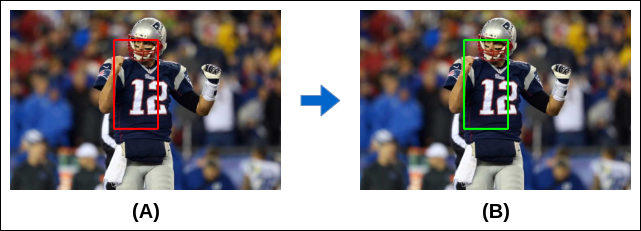
\includegraphics{6-Desenvolvimento-Projeto/imagens-desenvolvimento/representacao_numero.png}}
	\end{center}
	\centering \legend{Fonte: Elaborada pelos autores.}
\end{figure}

\begin{figure}[ht]
	\caption{\label{fig_rep_jogador_em_campo}Identificação de um jogador em uma partida de futebol americano.}
	\begin{center}
		\resizebox{.9\linewidth}{!}{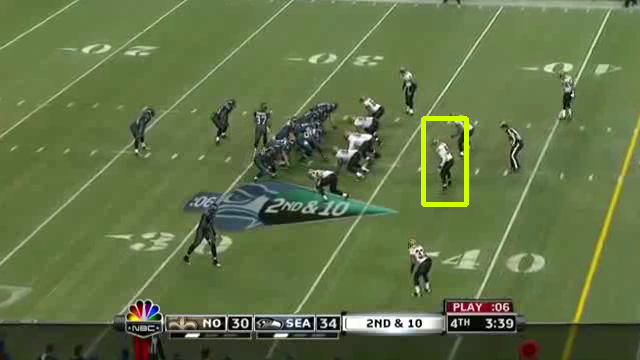
\includegraphics{6-Desenvolvimento-Projeto/imagens_teste/identificacao_jogador_em_campo_2.png}}
	\end{center}
	\centering \legend{Fonte: Elaborada pelos autores.}
\end{figure}

\begin{figure}[ht]
	\caption{\label{fig_rep_jogador_mais_evidente}Identificação do jogador mais evidente.}
	\begin{center}
		\resizebox{.9\linewidth}{!}{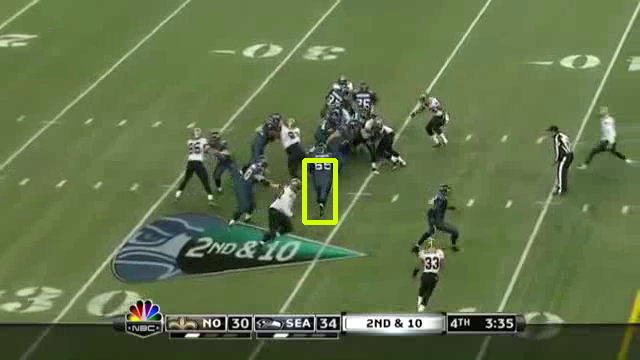
\includegraphics{6-Desenvolvimento-Projeto/imagens_teste/jogador_mais_evidente.png}}
	\end{center}
	\centering \legend{Fonte: Elaborada pelos autores.}
\end{figure}

\begin{figure}[ht]
	\caption{\label{fig_rep_jogador_em_movimento}Identificação de um jogador em movimento dentro de campo.}
	\begin{center}
		\resizebox{.9\linewidth}{!}{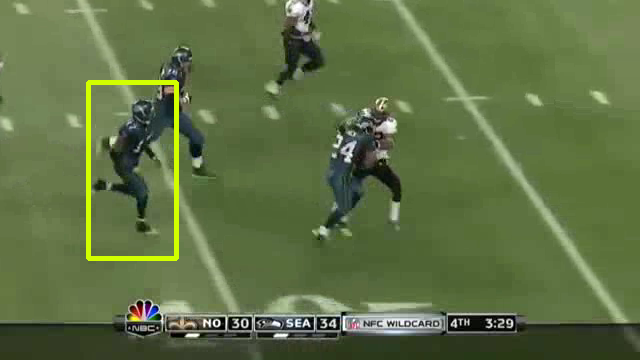
\includegraphics{6-Desenvolvimento-Projeto/imagens_teste/jogador_em_movimento.png}}
	\end{center}
	\centering \legend{Fonte: Elaborada pelos autores.}
\end{figure}

\begin{figure}[ht]
	\caption{\label{fig_rep_jogador_em_jogada}Identificação de um jogador em movimento para disputar uma jogada.}
	\begin{center}
		\resizebox{.9\linewidth}{!}{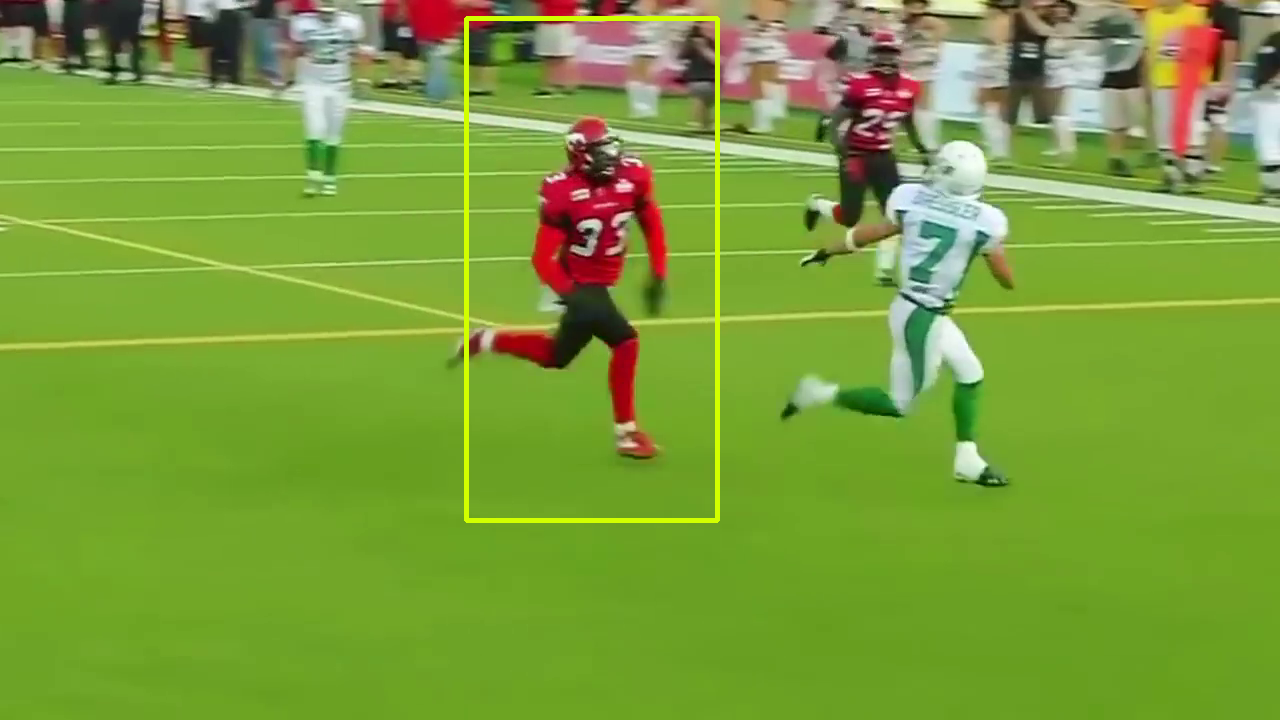
\includegraphics{6-Desenvolvimento-Projeto/imagens_teste/identificacao_jogadores_fa3.png}}
	\end{center}
	\centering \legend{Fonte: Elaborada pelos autores.}
\end{figure}

\begin{figure}[ht]
	\caption{\label{fig_rep_acessorios}Identificação dos acessórios de um jogador de futebol americano.}
	\begin{center}
		\resizebox{.9\linewidth}{!}{\includegraphics{6-Desenvolvimento-Projeto/imagens_teste/identificacao_jogadores_fa5.png}}
	\end{center}
	\centering \legend{Fonte: Elaborada pelos autores.}
\end{figure}

\begin{figure}[ht]
	\caption{\label{fig_rep_arbitro}Reconhecimento do árbitro dentro de campo.}
	\begin{center}
		\resizebox{.9\linewidth}{!}{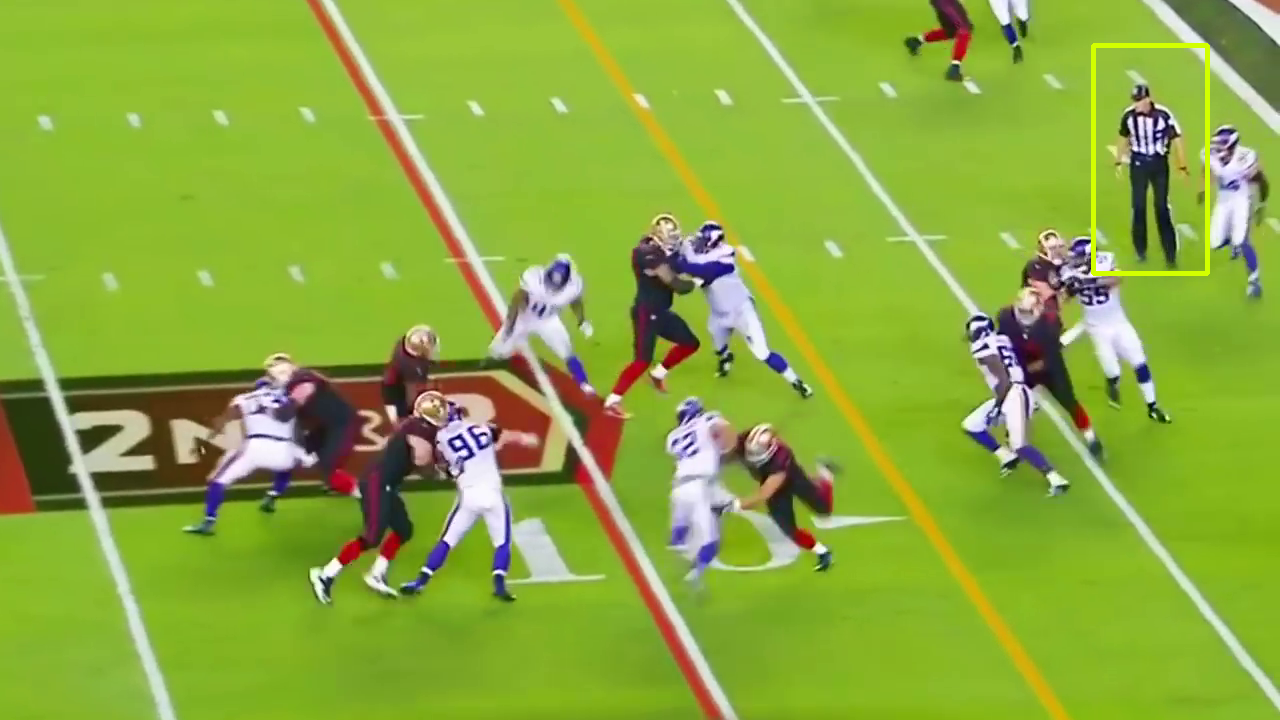
\includegraphics{6-Desenvolvimento-Projeto/imagens_teste/identificacao_arbitro.png}}
	\end{center}
	\centering \legend{Fonte: Elaborada pelos autores.}
\end{figure}

\begin{figure}[ht]
	\caption{\label{fig_processamento_maquina}Representação do processamento da máquina.}
	\begin{center}
		\resizebox{.9\linewidth}{!}{\includegraphics{6-Desenvolvimento-Projeto/imagens_teste/processamento_maquina.png}}
	\end{center}
	\centering \legend{Fonte: Elaborada pelos autores.}
\end{figure}

\clearpage